\chapter{Afgeleide klasse en objecten in C++}

Bij deze opdracht richten we ons hoe bij OO componenten Overerving en Polymorfisme getest kunnen worden met een debugger.

Deze opdracht bestaat verder uit de deelopdrachten A en B en er moeten 6 screenshots gemaakt worden die op brightspace moeten worden geüpload. Alle deelopdrachten moet je laten aftekenen door de docent.

Er zijn diverse soorten LEDs, zoals in figuur \ref{fig:LEDs} te zien zijn. Deze zijn:
\begin{itemize}
	\item SingleLed: deze LEDs hebben 1 kleur, twee pootjes en worden aan 1 poort op de RockPi aangesloten, zoals de rode, oranje en groene LED. Een voorbeeld wordt weergegeven in figuur \ref{fig:singleLed}
	\item DualLed: deze LEDs hebben 2 mogelijke kleuren, drie pootjes en worden aan 2 poorten (1 per kleur) aan de RockPi verbonden. Een voorbeeld wordt weergegeven in figuur \ref{fig:dualLed}
	\item RGB Led: deze LEDs hebben de kleuren rood, groen en blauw in 1 behuizing en hebben vier pootjes, waarvan 3 worden aangesloten op de poorten (1 per kleur) van de RockPi.De LED met de witte kleur op het practicumboord is een RGB LED. Een voorbeeld van een RGB LED wordt weergegeven in figuur \ref{fig:rgbLed}
\end{itemize}

\begin{figure}[h!]
	\centering
	\begin{subfigure}[b]{0.3\textwidth}
		\centering
		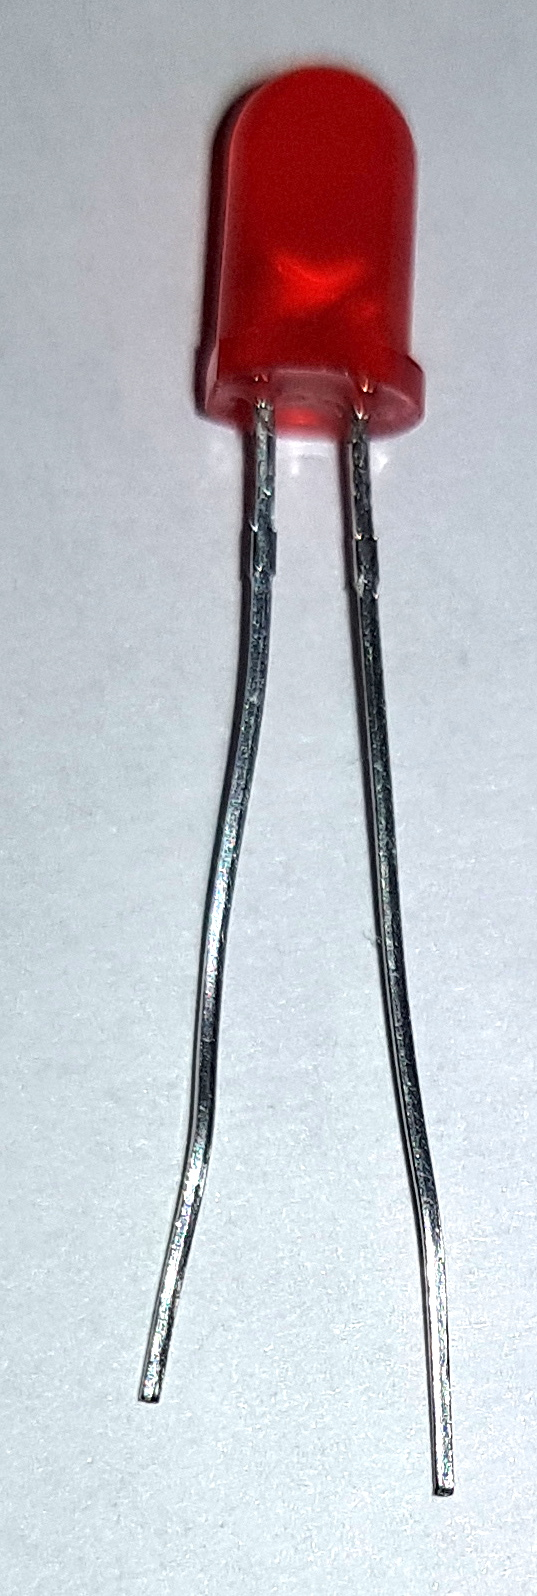
\includegraphics[width=0.7\textwidth,height=3.5cm]{figuren/singleled}
		\caption{een single LED}
		\label{fig:singleLed}
	\end{subfigure}
	\hfill
	\begin{subfigure}[b]{0.3\textwidth}
		\centering
		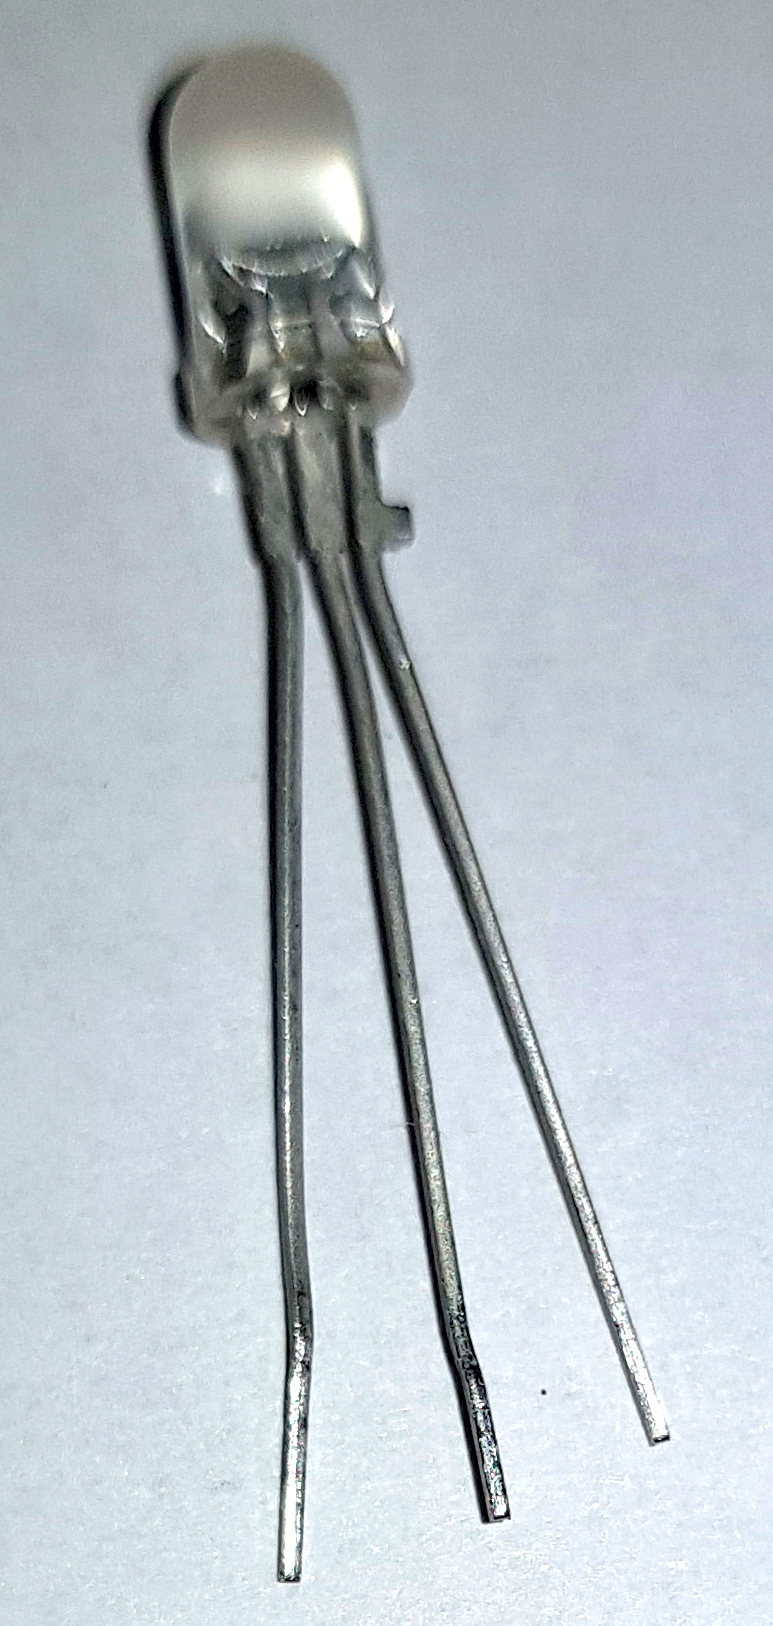
\includegraphics[width=0.7\textwidth,height=3.5cm]{figuren/dualled}
		\caption{een dual LED}
		\label{fig:dualLed}
	\end{subfigure}
	\hfill
	\begin{subfigure}[b]{0.3\textwidth}
		\centering
		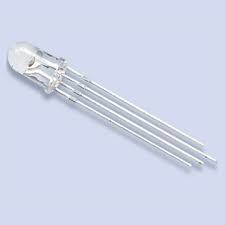
\includegraphics[width=0.9\textwidth,height=3.5cm]{figuren/rgbled}
		\caption{een RGB LED}
		\label{fig:rgbLed}
	\end{subfigure}
	\caption{Verschillende type LEDs}
	\label{fig:LEDs}
\end{figure}

De analist die de eisen voor de controller-software voor de LED controllers opstelt, heeft bedacht dat het in de toekomst mogelijk moet kunnen zijn om nieuwe LED types toe te voegen, bijvoorbeeld 3 kleuren LEDS. De controller software moet dus zo veel mogelijk onafhankelijk van het concrete LED type gemaakt worden. In figuur \ref{fig:klassLed} wordt de UML weergave geaan van zowel de SingleLed als de RGBLed
\begin{figure}[h!]
	\captionsetup{justification=centering}
	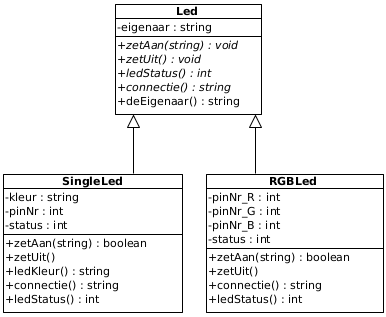
\includegraphics[width=0.6 \linewidth]{figuren/rgbKlasse}
	\centering
	\caption{De afgeleide klassen singleLed en RGBLed .}
	\label{fig:klasAfg}
\end{figure}
\newpage
De werking is als volgt.

\begin{itemize}
	\item Een LED wordt aangezet door de methode bool zetAan(string k); waarbij de parameter de kleur is die aangezet moet worden.
	\begin{itemize}
		\item Wordt bij een groene LED ''groen''  meegegeven, wordt de LED aangezet en true geretourneerd.
		\item Wordt bij een groene LED ''rood'' meegegeven, wordt de LED niet aangezet en wordt false geretourneerd.
	\end{itemize}
\item Een LED wordt uitgezet door de methode void zetUit(); Dit houd in dat bij een RGBLed alle kleuren uitgezet worden.
\item De methode string connectie(); geeft het gpioNummer van het aangesloten platform mee terug. In het geval van de RGBLed wordt een string mee teruggegeven met alle drie de gpioNummers gescheiden door een spatie.
\item Doordat de status van de LED verschillend zijn (een singleLed kan alleen aan en uit terwijl bij de RGBLed kan kleur1, kleur 2, kleur 3 of een combinatie van kleuren aan- en uitgaan), heeft elke afgeleide LED een eigen status.
\item Omdat bij een RGBLed al bekend is, wat de kleuren zijn (Rood, Groen en Blauw), hoef de kleur van de LED niet opgevraagd te worden. In tegenstelling tot een singleLed die maar \'{e}\'{e}n kleur heeft, dit kunnen overigens verschillende kleuren zijn.
\end{itemize}

%\paragraph{Opdracht} 
\section{De Klasse SingleLed}

Zoals in figuur \ref{fig:klasAfg} wordt aangegeven is de singleLed een speciale vorm van Led. Dit is ook terug te zien in de code, zoals Listing \ref{lst:singleLedH} laat zien.

\noindent\begin{minipage}{.45\textwidth}
\begin{lstlisting}[caption=LED declaratie file(.h),frame=tlrb,label={lst:ledBaseH}]{Name}
class Led
{
	public:
	/*
	
	Implementeer hier 
	de construcor(s) 
	en de methoden
	
	*/
	
	
	private:
       string eigenaar;
};
\end{lstlisting}
\end{minipage}\hfill
\begin{minipage}{.45\textwidth}
\begin{lstlisting}[caption=SingleLed declaratie file(.h),frame=tlrb,label={lst:singleLedH}]{Name}
class SingleLed : public Led
{
	public:
	/*
	
	Implementeer hier 
	de construcor(s) 
	en de methoden
	
	*/
	
	private:
        string kleur;
	    int pinNr;
	    int status;
};
\end{lstlisting}
\end{minipage}
\paragraph{Opdracht} 
\begin{enumerate}[label=(\alph*)]
\item
Implementeer de klasse Led en SingleLed (zowel de .h als de .cpp file )en run de main code van Listing \ref{lst:mainSled}.

\begin{lstlisting}[caption=main functie om de klasse SingleLed te testen. ,frame=trbl,firstnumber=1,numbers=left,label={lst:mainSled}]{Name}

void LedInfo(Led& l) {
	cout<<"De eigenaar is:"<<l.deEigenaar()<<endl;
	cout<<"De Led is aangesloten op pinnen"<<l.connectie()<<endl;
	cout<<"De status van de Led is:"<<l.ledStatus()<<endl;
}

int main() {
	
	SingleLed led1(RODELED,"rood","Pietje Puk");
	SingleLed led2(RODELED,"rood");
	
	Led &lr1(led1);
	lr1.zetAan("rood");
	usleep(1000000);
	led2.zetAan("geel"); 
	usleep(1000000);
	led1.zetUit();
	usleep(1000000);
	
	LedInfo(led1);
	LedInfo(led2);
	LedInfo(lr1);
	
	led2.zetUit();
	return 0;
}

\end{lstlisting}

De uitkomst van het programma wordt weergegeven op de volgende bladzijde.
\newpage
De eigenaar is:Pietje Puk\\
De Led is aangesloten op pinnen135\\
De status van de Led is:0\\
De eigenaar is:Anoniem\\
De Led is aangesloten op pinnen134\\
De status van de Led is:1\\
De eigenaar is:Pietje Puk\\
De Led is aangesloten op pinnen135\\
De status van de Led is:0\\
\item 
\begin{itemize}
	\item Start de vnc viewer op met hierin de ddd debugger.
	\item Plaats een breakpoint op regel 21 van Listing \ref{lst:mainSled} (LedInfo(led1)).
	\item Run het programma, de debugger zal stoppen op regel 21.
	\item Toon de objecten led1 en led2, zoals getoond in figuur \ref{fig:dddLed1_2}. 
	\begin{figure}[h!]
		\captionsetup{justification=centering}
%		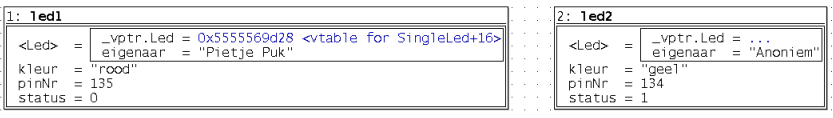
\includegraphics[width=0.95 \linewidth]{figuren/dddLed1Led2}
    	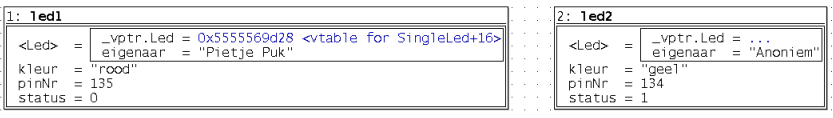
\includegraphics[width=0.95 \textwidth]{figuren/dddLed1Led2}
		\centering
		\caption{De inhoud van objecte led1 en led2 .}
		\label{fig:dddLed1_2}
	\end{figure}
	De tekst achter \texttt{\_vptr.led} kan verborgen worden door deze te selecteren en in de pull-down menu \textit{hide All} te kiezen. Hierin is duidelijk te zien dat de base-klasse  \textbf{Led} een onderdeel is van de afgeleide klasse \textbf{SingleLed}.
\end{itemize}

\item Maak een screenshot van beide objecten in de DDD debugger, uiteraard met je \textcolor{red}{\huge{eigen}} naam en plaatst deze met de \textbf{code} in je portfolio onder het hoofdstuk programmeren.

\end{enumerate}

\section{De Klasse RGBLed}

